\documentclass[11pt,a4paper,reqno]{amsart}
\usepackage[T1]{fontenc}
\usepackage[utf8]{inputenc}
\usepackage{lmodern,amssymb}
\usepackage[textwidth=160mm,textheight=235mm,centering,headheight=12pt,headsep=18pt]{geometry}
\usepackage{microtype,graphicx,xcolor,needspace}
% Alphabetic citation labels are defined explicitly in the bibliography.
\definecolor{linkblue}{RGB}{0,60,150}
\usepackage[colorlinks=true,linkcolor=linkblue,citecolor=linkblue,urlcolor=linkblue,bookmarksnumbered=true]{hyperref}
\makeatletter
\renewcommand{\@biblabel}[1]{[\textcolor{linkblue}{#1}]}
\def\ps@mathpaper{%
  \let\@mkboth\markboth
  \def\@oddhead{\normalfont\scriptsize
    \makebox[\textwidth][c]{\shorttitle}\llap{\thepage}}%
  \def\@evenhead{\normalfont\scriptsize
    \rlap{\thepage}\makebox[\textwidth][c]{\MakeUppercase{\shortauthors}}}%
  \let\@oddfoot\@empty
  \let\@evenfoot\@empty}
\makeatother
\pagestyle{mathpaper}
\AddToHook{cmd/section/before}{\Needspace{7\baselineskip}}
\numberwithin{equation}{section}
\renewcommand{\topfraction}{0.9}
\renewcommand{\textfraction}{0.08}
\renewcommand{\floatpagefraction}{0.8}
\setlength{\emergencystretch}{2em}
\clubpenalty=10000
\widowpenalty=10000
\raggedbottom
\hypersetup{pdftitle={Market for Formally Verifiable Work},pdfauthor={Yangyang Li, Jiaqi Lai, Xinze Li}}

\title{Market for Formally Verifiable Work}
\author{Yangyang Li}
\author{Jiaqi Lai}
\author{Xinze Li}
\date{}

% Active local manuscript: AMS layout with alphabetic citations.
% Text baseline: Overleaf 3e8c7b3, matching the user's Downloads/MathMarket.pdf.
% Version provenance and source checks: see resources/version_audit.md.
% CloK is discussed through its proposed use in this framework.
% No implemented integration or demonstrated forecast performance is asserted.
% Keep roles_interactions.pdf in the same directory as this source file.
\begin{document}
\maketitle

\section{Introduction}
AI agents can explore proof strategies and work on separate lemmas, while formal proof assistants check the resulting proofs. The human effort and computation needed to find a proof remain uncertain. Verification can establish whether a submitted argument proves the stated claim, but it does not tell us which unfinished attempts to fund.

Grants support exploration, whereas prizes reward completed results. When many researchers and agents pursue related tasks, funding decisions must also respond to intermediate results and new information. Which attempts should receive support? How should contributors be paid when their lemmas are useful but the main theorem remains open?

We propose a basic economic framework connecting demand, funding, proof work, verification, and settlement. Within this framework, we compare exploration support, intermediate rewards, and shared terminal prizes, and analyze how forecasts and competition affect investment decisions. Based on this analysis, we identify questions for future research, including the game-theoretic interactions among participants and the design of funding and reward mechanisms. Our examples come from mathematics, but the framework applies to any work whose acceptance can be checked formally, including verified software, hardware, and security properties.

\begin{figure}[htbp]
\centering
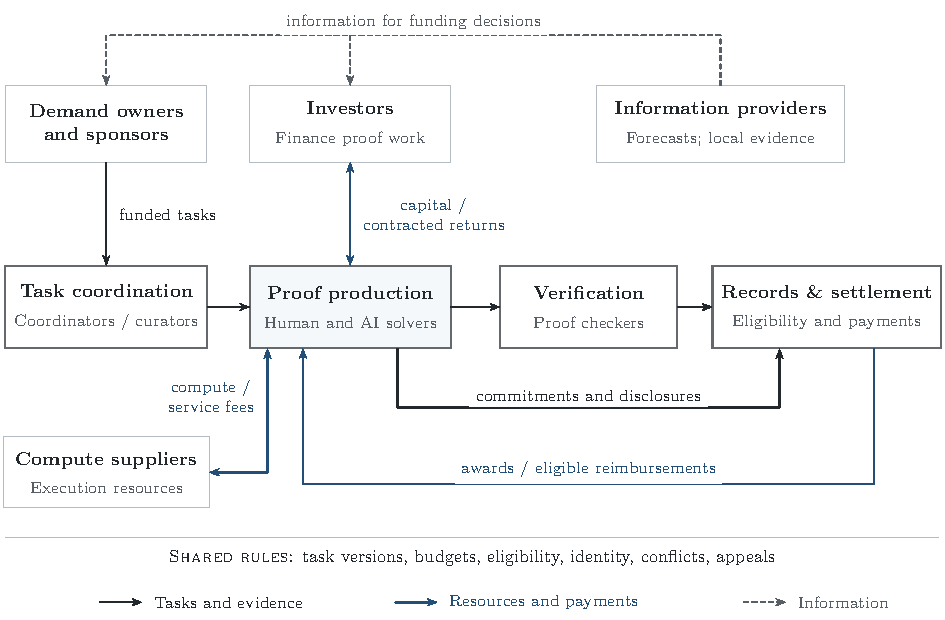
\includegraphics[width=\linewidth]{roles_interactions.pdf}
\caption{Principal relations among roles. The central row follows tasks and proof evidence; funding, information, and compute support this work. Records and eligibility rules govern payments separately from proof verification. Two-way arrows denote exchanges. One institution may perform several roles, and several institutions may share a role.}
\label{fig:roles}
\end{figure}

\section{Economic framework, funding, and investment}
\label{sec:framework}
Demand may come from a research community, a company, or an individual crypto patron. A sponsor values the result or its applications; an investor seeks a financial return from the work it finances. The framework permits conventional payments or cryptocurrency.

Solvers include human researchers, AI agents, and mixed teams. Coordinators define tasks and manage dependencies; verifiers check submitted proofs; settlement services distribute rewards. Compute suppliers provide execution resources, and information providers help participants assess ongoing work. A task specifies the statement, acceptance criteria, budget, and reward rules before work begins. The statement may be a mathematical theorem or a formal specification that software, hardware, or a protocol must satisfy.

These roles are not mutually exclusive. A solver may also act as an investor, financing work on some lemmas while proving and integrating others. Delegating a lemma to another participant may reduce costs or shorten completion time, particularly when participants have different expertise or computational resources. Compensation may take the form of a fixed payment or a share of the eventual award.

\subsection{Exploration support}
Advance compute credits fund approved searches before work begins; capped reimbursement covers eligible expenses afterward. Credits reduce the need for upfront funding but restrict provider choice. Reimbursement offers more flexibility but requires participants to front costs and accept audit delays. Both need committed budgets, spending limits, and checks against duplicate claims.

Reimbursement requires records linking the claimed expenses to the approved task. An unsuccessful attempt may still qualify for support, but support should pay for bounded exploration, not failure itself.

\subsection{Intermediate rewards}
An approved lemma can carry its own reward, paid when its proof is accepted even if the main theorem remains unresolved. Specialized contributors can then work on individual dependencies. Separate budgets can reward integration and reuse. Reviewing tasks before assigning awards can discourage artificial fragmentation. A reduction that assumes unresolved lemmas does not complete the main theorem.

\subsection{Priority and shared rewards}
A fixed terminal prize can go to the first eligible submission or be shared among eligible submissions committed within an announced window. A shared commitment phase followed by proof disclosure limits copying from those disclosures. Sharing can recognize near-simultaneous work but reduces each winner's payment and can encourage duplicate claims through multiple accounts. Contracts must specify timing, eligibility, and whether rewards attach to a participant, team, or distinct contribution.

\subsection{Investment under heterogeneous beliefs}
Investor $i$ evaluates action $a$ using information $\mathcal I_{i,t}$ and subjective beliefs $Q_{i,t}$:
\begin{equation}
\label{eq:expected-return}
 \Pi_{i,t}(a)=\mathbb E_{Q_{i,t}}\!\left[
 R_i(a)-C_i^{\mathrm{net}}(a)\mid\mathcal I_{i,t}\right].
\end{equation}
Here $R_i$ denotes the investor's contracted receipts and $C_i^{\mathrm{net}}$ its costs after eligible support. Investors may disagree about the same task; liquidity and risk preferences also affect their decisions. Producing a valid proof, qualifying for payment, and earning a profit are different outcomes.

The action \(a\) may include proving a lemma directly, delegating it, or combining internal and external work. These choices involve tradeoffs among payments, coordination costs, and completion time. The expression above measures expected financial return; a participant's broader objective may also include scientific progress, timely completion, and recognition.

Expert assessments, forecasts, and local experiments inform these decisions. Their relevance depends on the task, proving procedure, budget, and horizon. Competition affects both the probability of receiving an award and the share paid to each successful contributor.

\section{Institutional examples and coordination}
\label{sec:examples}

As of this writing (October 2026), several functions identified in the framework above have taken concrete form in existing projects and institutional practices. We examine the roles these initiatives play in an emerging ecosystem for mathematical research, how they complement one another, and what coordination problems remain.

\subsection{Institutional funding and demand}
Government agencies, philanthropic foundations, and corporate sponsors provide organized channels for supporting mathematical research and infrastructure. DARPA's expMath program seeks AI systems that decompose mathematical problems and develop reusable lemmas~\cite{darpa}. The Simons Foundation supports researchers, institutions, and scientific infrastructure through its Mathematics and Physical Sciences division~\cite{simons}. Renaissance Philanthropy's AI for Math Fund, with XTX Markets as its founding donor, supports mathematical research, tools, and infrastructure~\cite{renaissance}. XTX Markets also reports support for Lean and mathlib~\cite{xtx}.

These arrangements support research capacity as well as particular results. AWS's use of automated reasoning for security illustrates corporate demand for verified capabilities~\cite{aws}. Such demand can motivate funded tasks, while institutional grants can support people and shared tools. The relevant distinction is how funding is organized and administered: foundations and companies also deploy private capital.

\subsection{Individual patronage and cryptocurrency prizes}
Individually initiated prizes provide a further route for sponsoring mathematics. The Justin Sun Prize is personally funded by Justin Sun and administered through a dedicated prize organization. Its rules announce a USD~1~million award for each qualifying problem in the highest tier and distinguish solving from Lean formalization contributions. Awards are denominated in dollars, with payment specified in USDT on TRON or USDC on Ethereum~\cite{sunclaims,sun}. The dollar thus provides the unit of account, while stablecoins provide the settlement asset.

The public award register already lists recognized solving and formalization contributions~\cite{sunawards}. Together with submission, verification, priority-review, and claim procedures, these records document an operating incentive scheme for mathematical results. Cryptocurrency-based sponsorship has therefore acquired concrete organizational form outside conventional mathematical prize institutions. Its effects on additional research effort and mathematical output remain empirical questions.

\subsection{CloK: forecasts for funding decisions}
In this framework, CloK would serve as an information provider. Its predictions could provide important information before a proof is available, when sponsors decide what to fund and investors choose which attempts to support. Relevant assessments concern a conjecture's truth, the resources needed to resolve it, and the further results that its resolution could enable.

Such information could help compare candidate lemmas, allocate compute among approaches, and revise funding as work progresses. An inexpensive lemma may unlock several costly tasks; a plausible conjecture may still be a poor short-term investment. Sponsors may prioritize mathematical value, while investors must also account for the reward and competing teams.

Using CloK's forecasts in this way requires relating them to a specified task, proving procedure, budget, and horizon. Confidence in a conjecture's truth is not the probability that a particular team will earn a reward. Forecasts would guide decisions about unfinished work, rather than replace verification afterward.

\subsection{OpenMath: token incentives and rewards for reuse}
OpenMath explores an arrangement built around CTK, Shentu's transferable native token, which is also traded on cryptocurrency exchanges~\cite{shentutoken,ctkmarket}. The platform uses CTK for theorem funding and proof rewards. Its documented interface integrates Web3-wallet authentication, transaction signing, and reward claims; users can publish funded statements and add funding to open theorems. Its agent tooling supports local Lean or Rocq proof work, followed by a proof-hash commitment, disclosure, and verification~\cite{openmath}. Wallet integration connects participation and proof submission to the account used to receive rewards.

The reward rules also account for reused results. In the published v2.19.0 implementation, an accepted proof triggers allocation from the theorem's funded pool: the checker receives a complexity-based amount, the proposers of referenced theorems receive reuse payments, and the current prover receives the remainder~\cite{openmathprotocol}. A referenced theorem's payment depends on its recorded complexity and prior import count. The recipient is its registered proposer, who need not be its proof author.

These arrangements make reward denomination and settlement infrastructure explicit elements of mechanism design. The Justin Sun Prize specifies dollar amounts for stablecoin settlement, whereas OpenMath embeds rewards in a native-token economy. For a contributor evaluating returns in dollars, a CTK reward's realized value depends on the exchange rate and liquidity at conversion. Reuse payments additionally connect intermediate results to later funding, raising questions about who holds the reuse claim and how complexity and reuse should be valued. Upfront exploration support and sharing among competing successful proofs remain separate design choices.

\subsection{PNT+ and Tau Ceti: community formalization}
The Prime Number Theorem and Beyond (PNT+) project, led by Alex Kontorovich and Terence Tao, pioneered the crowdsourcing of mathematics through formal verification. Its blueprint divides the target results into separately stated lemmas; contributors claim individual tasks through the project's issue tracker, coordinate on the Lean Zulip, and submit proofs that Lean checks~\cite{pnt}. The proof assistant, rather than trust in each contributor, confirms that the pieces fit together.

Tau Ceti, incubated by the Lean FRO and the Mathlib Initiative, extends this division of labor to AI contributors. Mathematicians and formalization experts write roadmaps; AI agents implement the formal mathematics, and other AI agents review each contribution adversarially against rubrics written by humans. The library builds on Mathlib without duplicating it and was reported in October 2026 to be slightly larger than Mathlib~\cite{tauceti,taucetipost}. Contributors supply roadmaps or pay the inference costs of their own pull requests; the organizers have announced financial models for the project but not yet published them~\cite{taucetipost}.

These projects show that coordination and verification can operate at scale without task-level payments. Blueprints and roadmaps perform the coordinator's role in our framework. Review rubrics address what a proof checker alone cannot: whether a formal statement says what was intended. Attaching payments to such tasks would add questions of eligibility and attribution, which the remaining examples address in different ways.

\subsection{Prove2Me: collaborative formalization}
Prove2Me provides infrastructure for collaborative formalization by human contributors and AI agents. A mission specifies a goal, its definitions, and selected milestone lemmas for human audit. Proof sketches express the goal's dependence on separately stated lemmas, allowing agents to work on different parts of the argument; completion requires closing the necessary dependencies. Proved results can be searched and imported across missions. The platform records credit both for completing proofs and for proposing statements that later proofs reuse~\cite{prove2me}.

The platform played a central role in the Fermat's Last Theorem formalization reported by Anthropic in September 2026. Using Prove2Me and a Claude Code-based multi-agent system, Claude agents produced a complete Lean formalization in 11 days, with approximately 13 million lines of code and 29,500 intermediate theorems used in the final proof. Prove2Me supplied dependency tracking, compilation support, and theorem search and reuse. The development also incorporated work from Mathlib, the Imperial College FLT project, and the regular-prime formalization~\cite{anthropicflt}. This provides a concrete example of coordinating many local proof contributions into a verified mathematical result.

In our framework, mission milestones and recorded dependencies could serve as units for allocating compute, sponsoring intermediate lemmas, and attributing contributions. Funding could support separate proof tasks as well as their integration into a completed mission. Attaching rewards to these units would require committed budgets and contracts specifying eligibility and the division of payments among proof authors, integrators, and contributors of reused results. Contribution credit supplies an attribution record; payment rights would be defined by those contracts.

\subsection{Prediction markets: rewarding informed participants}
Prediction markets create opportunities to earn returns from information about future events~\cite{wolfers}. Consider a contract paying one unit if an accepted proof is published by a fixed deadline, and zero otherwise. A risk-neutral participant assigning probability $q$ to that event has a subjective expected profit of $q-p$ when buying at price $p$, before fees and financing costs. Better-informed participants may profit by identifying mispriced contracts, while mistaken judgments can incur losses. These incentives can encourage information gathering and bring dispersed knowledge into market prices.

In mathematics, research insiders may understand a promising approach, a difficult dependency, or the capabilities of a proving system before that information is widely appreciated. A market that permits their participation could reward this knowledge through trading returns, including when they do not submit the final proof. For example, someone who recognizes an overlooked obstruction could profit from a contract paying on non-completion. Their trades could help sponsors and investors revise funding decisions. This provides a possible source of compensation for information providers, alongside rewards for producing mathematical results.

Exchanges such as Kalshi illustrate event-based settlement: its filed Millennium Prize contract concerns an official award announcement by the Clay Mathematics Institute~\cite{kalshi}. A market for proof completion would need its own acceptance criteria and deadline. Participation rules also shape the incentive mechanism: Kalshi prohibits insider trading and trading by people able to influence the outcome~\cite{kalshirules}. Rewarding research insiders is therefore a design question for a proposed research market. It requires deciding which information and participants are eligible, how trading relates to disclosure, and how to prevent positions on non-completion from rewarding the withholding or obstruction of progress.

\subsection{Coordination across institutions}
Connecting these functions requires common task identifiers and versions, reproducible verification environments, authenticated submission records, and reconciled payment claims. A lemma-level forecast, the funded task, and the submitted proof must refer to compatible statements and assumptions. Contracts must specify who may revise tasks, decide eligibility, and resolve disputes; each payment claim must be redeemable only once. Independent review matters when an institution both finances a solver and judges its award. Shared records can support priority and settlement, but cannot establish independent discovery.

\section{Future research}
\label{sec:research}

\subsection{Game theory and mechanism design}
A game-theoretic model should take individuals, teams, or institutions as players, rather than the roles themselves. Each player has its own objectives and may perform several roles. A team may pursue a theorem, finance delegated lemmas, and compete for rewards on other tasks. Its decisions reflect its objectives across these activities, which may include financial return, scientific progress, completion time, and reputation.

A natural next step is to study a dynamic game with incomplete information about task difficulty, capabilities, costs, and private progress. Players choose what to prove themselves, what to delegate, whom to collaborate with, and when to disclose results. When does delegation reduce total cost or accelerate completion? When does competition support complementary work rather than duplication? Which contracts and reward rules encourage participants with different objectives to share useful results?

\subsection{Forecasts, entry, and disclosure}
A favorable forecast, including one supplied by CloK, may attract funding and additional solvers. This can raise the chance of completing a mission while reducing individual returns through competition. How should allocation rules respond to this feedback? How should information providers be rewarded when their forecasts influence the outcomes being predicted? What disclosure and conflict-of-interest rules are needed when forecasters also invest in or work on the tasks they assess?

These questions also concern correlated mistakes. When many participants rely on similar models or forecasts, apparently separate investments may support the same unsuccessful strategy. A model of investment should account for shared methods and proof dependencies, not only the number of funded tasks.

\subsection{Empirical evaluation}
Controlled comparisons should hold total budgets fixed while varying exploration support, lemma rewards, terminal prize rules, and disclosure schedules. Outcomes should include accepted and reused results, completion times, total compute and review costs, participation, duplicate work, and disputed payments. Results reused across missions should be recorded so that benefits and costs are not counted as independent.

Forecasts should be recorded before attempts begin. A CloK-informed allocation policy could then be compared with expert selection, equal allocation among eligible tasks, and policies based on local proof experiments. Evaluation should include unsuccessful attempts and account for censoring in stopped or unfinished runs. Prediction accuracy and decision quality should be measured separately: the central question is whether forecasts improve the allocation of resources and the mathematical progress those resources produce.

\begin{thebibliography}{CML$^{+}$26}
\setlength{\itemsep}{3pt}
\bibitem[ABC$^{+}$26]{taucetipost} Jeremy Avigad, Kevin Buzzard, Johan Commelin, R\'emy Degenne, Kim Morrison, Oliver Nash, and Adam Topaz. ``How to Formalize All of Mathematics.'' \emph{Xena Project} (blog), October~16, 2026. \href{https://xenaproject.wordpress.com/2026/10/16/how-to-formalize-all-of-mathematics/}{Guest post}.
\bibitem[Ant26]{anthropicflt} Anthropic. \emph{Formalizing Fermat's Last Theorem}. September~4, 2026. \href{https://www.anthropic.com/news/formalizing-fermats-last-theorem}{Official research report}; \href{https://github.com/anthropics/fermats-last-theorem}{published Lean proof and verification documentation}.
\bibitem[AWS]{aws} Amazon Web Services. \emph{Provable Security}. Undated. \href{https://aws.amazon.com/security/provable-security/}{Official overview}. Accessed October~14, 2026.
\bibitem[Bin]{ctkmarket} Binance. \emph{CTK/USDT Spot Market}. Undated. \href{https://www.binance.com/en/trade/CTK_USDT?type=spot}{Exchange market page}. Accessed October~14, 2026.
\bibitem[CML$^{+}$26]{prove2me} Shuze Chen, Kunal Marwaha, Xiaoyang Lu, Henry Yuen, and Tianyi Peng. \emph{Prove2Me: An Open Collaborative Platform for Scaling Math Formalization}. \href{https://arxiv.org/abs/2608.28433v2}{arXiv:2608.28433v2}, August~31, 2026. DOI: \href{https://doi.org/10.48550/arXiv.2608.28433}{10.48550/arXiv.2608.28433}.
\bibitem[DARPA]{darpa} DARPA. \emph{expMath (Exponentiating Mathematics)}. Undated. \href{https://www.darpa.mil/research/programs/expmath-exponential-mathematics}{Official program description}. Accessed October~14, 2026.
\bibitem[JSPa]{sunawards} The Justin Sun Prize. \emph{Confirmed Awards}. Undated. \href{https://github.com/TheJustinSunPrize/awards/blob/fd8fa66abb4e21df828fdebc25298e9ad75521bd/awards/README.md}{Official award register}, repository snapshot \texttt{fd8fa66}. Accessed October~14, 2026.
\bibitem[JSPb]{sunclaims} The Justin Sun Prize. \emph{Prize Claim Guidelines}. Undated. \href{https://www.hejustinsun.com/prize/claim}{Official procedures}, sections~I--IV. Accessed October~14, 2026.
\bibitem[JSPc]{sun} The Justin Sun Prize. \emph{Justin Sun Prize Selection Rules}. Undated. \href{https://www.hejustinsun.com/prize/rules}{Official rules}, sections~2.1, 3.1, 3.3, 4.1, and~5. Accessed October~14, 2026.
\bibitem[Kal]{kalshirules} Kalshi. \emph{Stopping Insider Trading}. Undated. \href{https://kalshi.com/policy-center/insider-trading}{Official policy overview}. Accessed October~14, 2026.
\bibitem[KEX25]{kalshi} KalshiEX LLC. \emph{Will a Millennium Prize Be Awarded Before $\langle\mathrm{date}\rangle$?} \href{https://www.cftc.gov/filings/ptc/ptc08142528943.pdf}{Contract filing}, August~14, 2025, Appendix~A.
\bibitem[KT]{pnt} Alex Kontorovich, Terence Tao, et al. \emph{PrimeNumberTheoremAnd}. Undated. \href{https://github.com/AlexKontorovich/PrimeNumberTheoremAnd}{Project repository}, with blueprint and contributing guide. Accessed October~21, 2026.
\bibitem[RP]{renaissance} Renaissance Philanthropy. \emph{AI for Math Fund}. Undated. \href{https://www.renaissancephilanthropy.org/ai-for-math-fund/}{Official fund description}. Accessed October~14, 2026.
\bibitem[SFa]{openmath} Shentu Foundation. \emph{OpenMath Learn Doc} and \emph{OpenMath Skills Arena}. Undated. \href{https://github.com/shentufoundation/docs/blob/main/docs/openmath/openmath-learn-doc.md}{Official user documentation}, sections~2, 4--6; \href{https://github.com/shentufoundation/openmath-skills}{agent tooling}. Accessed October~14, 2026.
\bibitem[SFb]{shentutoken} Shentu Foundation. \emph{Shentu Chain Whitepaper}. Undated draft. \href{https://shentu.org/whitepaper}{Official whitepaper}, section~1.2, ``CTK Coin and Economic Model.'' Accessed October~14, 2026.
\bibitem[SF26]{openmathprotocol} Shentu Foundation. \emph{Shentu v2.19.0}. Software, 2026. \href{https://github.com/shentufoundation/shentu/blob/v2.19.0/x/bounty/keeper/funds.go}{OpenMath reward allocation}; \href{https://github.com/shentufoundation/shentu/blob/v2.19.0/x/bounty/keeper/msg_server.go}{proof acceptance and theorem creation}. Accessed October~14, 2026.
\bibitem[Sim]{simons} Simons Foundation. \emph{Mathematics \& Physical Sciences}. Undated. \href{https://www.simonsfoundation.org/mathematics-physical-sciences/}{Official division overview}. Accessed October~14, 2026.
\bibitem[TCP]{tauceti} Tau Ceti Project. \emph{Tau Ceti}. Undated. \href{https://github.com/TauCetiProject/TauCeti}{Project repository}; \href{https://taucetiproject.org}{project website}. Accessed October~21, 2026.
\bibitem[WZ04]{wolfers} Justin Wolfers and Eric Zitzewitz. ``Prediction Markets.'' \emph{Journal of Economic Perspectives} 18(2): 107--126, 2004. DOI: \href{https://doi.org/10.1257/0895330041371321}{10.1257/0895330041371321}.
\bibitem[XTX26]{xtx} XTX Markets. \emph{Update on XTX Markets' AI for Maths Philanthropy}. September~16, 2026. \href{https://about.xtxmarkets.com/news/2026-update-on-xtx-markets-ai-philanthropy/}{Official announcement}. Accessed October~14, 2026.
\end{thebibliography}

\end{document}
